\subsubsection{Stufenindex (SI-POF)}

Der Stufenindex ist durchsatzschwächste Brechzahlprofil (ca. 100 Megabit/s auf
100 m, spezielle Übertragungsverfahren erlauben Bitraten im Bereich von 1
Gigabit/s). Als Kernmaterial wird Polymethylmethacrylat (PMMA, siehe
\autoref{subsec:pofpmma}) mit einem Durchmesser von ca. 1 mm, welcher von einem
ca. 10 µm Mantel umgeben ist, eingesetzt \cite{pofacsi}. \autoref{fig:pofsi}
fasst den Aufbau und die Lichtausbreitung zusammen. Die Spalte mit
Brechungsindex als Überschrift stellt den Verlauf dieses grafisch dar. Beim
Stufenindexprofil steigen die Brechzahlen beim Übergang vom Mantel zum Kern
abrupt an. Dies hat die schon erwähnte Totalreflexion an der Kerngrenze, welche
man in der Spalte Querschnitt erkennen kann, zur Folge.

\begin{figure}[h]
    \begin{center}
        \begin{minipage}[t]{0.4\textwidth}
            \begin{center}
                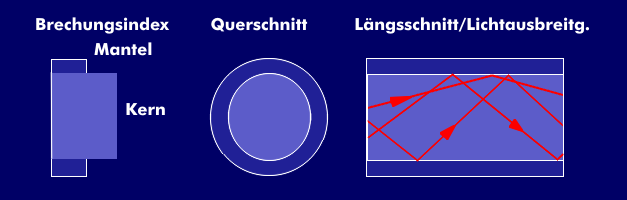
\includegraphics[width=0.9\textwidth]{Bilder/Optische_Wellenleiter_Die_Polymer_Optische_Faser/Brechzahlprofile/pofsi.png}
                \caption[Aufbau des Stufenindexprofils \newline \url{http://www.itwissen.info/bilder/aufbau-und-brechungsprofil-der-stufenindex-profilfaser.png} (zuletzt aufgerufen am 19.09.2015)]{Aufbau des Stufenindexprofils}
                \label{fig:pofsi}
            \end{center}
        \end{minipage}
        \hspace{0.025\textwidth}
        \begin{minipage}[t]{0.4\textwidth}
            \begin{center}
                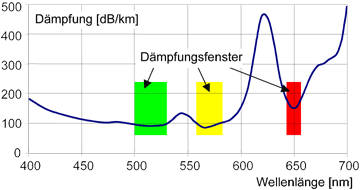
\includegraphics[height=0.1\textheight]{Bilder/Optische_Wellenleiter_Die_Polymer_Optische_Faser/Funktionsweise/pofdaempfung.png}
                \caption[Dämpfungsfenster bei einer polymer optischen Faser \newline \url{http://www.pofac.fh-nuernberg.de/pofac/de/was_sind_pof/images/pmma_daempfung.png} (zuletzt aufgerufen am 19.09.2015)]{Dämpfungsfenster beim Stufenprofil}
                \label{fig:pofdaempfung}
            \end{center}
        \end{minipage}
    \end{center}
\end{figure}

%TODO: enhance reference for sections

\autoref{fig:pofdaempfung} zeigt die Dämpfungsfenster einer polymer optischen
Faser. Diese liegen bei den Farben grün, gelb und rot. Um die Intensitätsabnahme
möglichst gering zu halten und damit die Reichweite zu erhöhen werden
Wellenlängen für die Lichtimpulse gewählt, die in den Dämpfungsfenstern liegen.
Als Lichtquelle kann zum Beispiel eine LED verwendet werden und als Empfänger
kommen Photodetektoren zum Einsatz. Der geringe Preis und die robuste
Übertragung auf kurzen Strecken machen die SI-POF zu einer beliebten alternative
gegenüber von Kupferkabeln in Industrieanlagen oder in Fahrzeugen. \cite{poflee}
